\documentclass[11pt,letterpaper]{article}
\usepackage[T1]{fontenc}
\usepackage[utf8]{inputenc}
\usepackage{newtxtext}
\usepackage[varqu,scaled=0.94]{zi4}
\usepackage{newtxmath}
\usepackage[margin=1in]{geometry}
\usepackage{microtype}
\usepackage{graphicx}
\usepackage{booktabs}
\usepackage{enumitem}
\usepackage{xcolor}
\usepackage{tikz}
\usetikzlibrary{arrows.meta}
\usepackage[font=small,labelfont=bf,skip=6pt]{caption}
\usepackage[numbers,sort&compress]{natbib}
\definecolor{linkblue}{HTML}{1F4E9E}
\newcommand{\papertitle}{Measure first: local scoring and training for small Gemma 4 coding agents}
\newcommand{\papersubtitle}{A sound local scorer, an out-of-distribution test set,\\ a reference-based editing tool and a LoRA training pipeline}
\newcommand{\paperauthor}{Nikhil Reddy Gogu}
\newcommand{\paperurl}{https://github.com/NikhilGogu/measure-first}

\usepackage[colorlinks=true,allcolors=linkblue,bookmarksnumbered=true,bookmarksopen=true,
  pdftitle={\papertitle},pdfauthor={\paperauthor},
  pdfsubject={Gemma 4 Developer Agent Competition, paper track},
  pdfkeywords={coding agents, small language models, evaluation, LoRA, software engineering}]{hyperref}
\usepackage{bookmark}

% no paragraph is split across pages; pages end on one baseline
\clubpenalty=10000 \widowpenalty=10000 \displaywidowpenalty=10000 \interlinepenalty=10000
\flushbottom
\setlength{\parindent}{0pt}
\setlength{\parskip}{0.5em plus 0.35em minus 0.1em}
\setlist{itemsep=0.25em plus 0.1em,topsep=0.2em,parsep=0pt,leftmargin=1.4em}
\setlength{\bibsep}{0.2em plus 0.2em}
\renewcommand{\bibfont}{\footnotesize\raggedright}
\setlength{\emergencystretch}{1.5em}
\hyphenation{sub-process fast-api py-dan-tic star-lette}
\makeatletter
\renewcommand{\paragraph}{\@startsection{paragraph}{4}{\z@}{0.2em plus 0.2em}{-0.6em}{\normalfont\normalsize\bfseries}}
\renewcommand{\section}{\@startsection{section}{1}{\z@}{1.1em plus 0.5em minus 0.2em}{0.35em plus 0.1em}{\normalfont\large\bfseries}}
\makeatother

\begin{document}
\begin{center}
  {\LARGE\bfseries \papertitle\par}
  \vspace{0.55em}
  {\large \papersubtitle\par}
  \vspace{1.2em}
  {\large \paperauthor\par}
\end{center}
\vspace{0.4em}

\begin{center}
\begin{minipage}{0.88\linewidth}
\small
\textbf{Abstract.}\enspace
The Gemma 4 Developer Agent competition scores an agent on hidden tasks from private repositories once a day, and the result arrives 8 to 33~hours later, so design choices rest on local measurement. I contribute four resources for it and report what they show for the small Gemma 4 E4B model. (1) A local scorer with per-task soundness controls: after three environment fixes, 50 of the 129 public tasks pass their reference fix and fail an empty patch in the Docker sandbox, and~69 in the subprocess sandbox. (2) An adapter that runs the unchanged agent loop on 86 newer tasks from 86 other repositories. (3) \texttt{cx}, a tool that edits code by reference: E4B resolves 7 of the 50 sound public tasks with it against~3 with the starter agent, and the 31B model 8 against~16. (4) A pipeline that turns verified runs into LoRA training data with the exact served tokens and~7 to 10~times fewer training tokens. Trained on a 31B teacher's runs, E4B loops; trained on its own verified runs it passes a loop screen, with gains inside run-to-run noise. Code and task lists are released under Apache~2.0.

\end{minipage}
\end{center}
\vspace{0.4em}

\section{Introduction}\label{sec:intro}

A coding agent built on a small open model can run on a developer's own hardware, but small models still lag on multi-turn repository work \citep{sweprotege}. The Gemma 4 Developer Agent competition \citep{g4comp} asks for such an agent. A submission is an agent configuration for the organisers' loop, one Gemma 4 checkpoint and optional LoRA adapters, and it must work through about 120 hidden tasks within 12~hours on four L4 GPUs. One submission a day is scored, and the score arrives 8 to 33~hours~later.

Under these limits almost every decision is made on local numbers, and a local number misleads in three ways. The scorer's environment can fail a correct fix, so the task measures nothing. The public tasks come from four repositories, while the hidden tasks come from private ones. Two identical runs differ by several~tasks.

This paper describes what I built against each and what it showed for Gemma 4 E4B (E4B below) and Gemma 4 31B (31B): a local scorer with soundness controls, an out-of-distribution task set that runs in the unchanged agent loop, \texttt{cx}, a reference-based code tool, a capture, packing and training pipeline for LoRA on agent runs, a time projection for the 12-hour budget, and a fine-tuning study with a decision rule fixed in advance, a loop screen and negative results (Sections 3~to~8).


\section{Related work}\label{sec:related}

\paragraph{Benchmarks and their validity.} SWE-bench \citep{swebench} scores a patch by running a repository's tests. An audit found leaked solutions and weak tests behind a large share of the patches it counts as resolved \citep{swebenchplus}. SWE-rebench \citep{swerebench} collects new tasks continuously, which keeps test tasks newer than a model's training data. Participants reported that this competition's reference patches fail locally for want of test dependencies \citep{forumdeps}, and one rebuilt a sandbox in which 127 of the 129 pass \citep{forumgold}. My controls add an empty-patch check in both of the scorer's sandboxes as shipped and identify two further~faults.

\paragraph{Agent interfaces.} SWE-agent \citep{sweagent} showed that the design of the tool interface changes how many issues a model resolves. \texttt{cx} is an interface for a small model: BM25 retrieval \citep{bm25} and edits addressed by~reference.

\paragraph{Training small agents.} SWE-Gym \citep{swegym} and SWE-smith \citep{swesmith} fine-tune open models on agent runs collected in executable environments. Imitating an expert's runs suffers from covariate shift \citep{oec}. Small models learn poorly from much stronger teachers \citep{learnability}, and small agents repeat actions \citep{deloop,sweprotege}. SWE-Ladder \citep{sweladder} and OPRD \citep{oprd} distil from a teacher that sees privileged evidence. My fine-tuning study meets the same failures inside the competition's loop and adds a cheap screen for them. Comparisons are paired on the same tasks, as \citet{errorbars}~recommends.


\section{A local scorer with soundness controls}\label{sec:scorer}

I run the scorer's own packages (swegemma 0.2.11, adk-submission 0.2.13, google-adk 1.36.1) and serve models with the official vLLM \citep{vllm} settings: gemma4 tool and reasoning parsers, 32,768-token context, tensor parallel 4 on four L4 GPUs. A local result counts only on tasks that pass two controls: the reference patch must resolve the task, and an empty patch must~not.

The first control run failed most fastapi tasks. Three faults were responsible, none of them in the agent; the first had been reported on the forum~\citep{forumdeps}:

\begin{itemize}
\item Test dependencies are installed with \texttt{-{}-no-deps}, so pydantic's \texttt{typing\_inspection} was missing and fastapi's reference fixes failed 66~of~67.
\item Every wheel under 20~MB is injected into every task container. The \texttt{inline\_snapshot} pytest plugin then loaded into rich's tests and broke them. Padding that wheel past 20~MB makes it load only where a task imports~it.
\item The unpacked-wheel cache is keyed by name only, so a changed wheel kept its old contents until the cache was~deleted.
\end{itemize}

After the fixes, 50 of the 129 public tasks are sound in the Docker sandbox: 38 of~48 from rich and~12 of~67 from fastapi. Every comparison below is paired on the same sound~tasks.

The organisers' scoring notebook uses the scorer's other backend, a subprocess sandbox with one virtual environment per task. With the wheels as shipped, 69~tasks are sound there on my machines (29 fastapi, 40 rich) and~71 inside a Kaggle notebook. In both places 55~tasks fail their own reference fix, so in a local run with the shipped wheels more than 40\% of the public tasks cannot separate two agents. One check against the real scorer: the competition's starter agent, which uses only the scorer's built-in tools (the recipe below), resolved 7 of the 129 public tasks locally with E4B (5.4\%) and~3 of the 58 hidden tasks on the public leaderboard split~(5.2\%).


\section{Out-of-distribution tasks in the scorer's own loop}\label{sec:ood}

The hidden tasks come from private repositories, while the public tasks come from four. I wrote an adapter that runs the scorer's unchanged agent loop inside SWE-rebench \citep{swerebench} task images: the repository moves from \texttt{/testbed} to \texttt{/workspace}, git history is rebuilt at the base commit, protected test files are reset after the agent finishes, the task's test patch is applied, and a task counts as resolved only when every \texttt{FAIL\_TO\_PASS} and \texttt{PASS\_TO\_PASS} test~passes.

From the 120 newest permissively licensed tasks, one per repository (created 24~Jan to 30~Apr~2025), 86 pass the same two controls. Four disjoint training pools (3,046~tasks) share no repository with this set and contain no task from the four public repositories (they do include sibling repositories such as textual and~starlette).


\section{\texorpdfstring{\texttt{cx}}{cx}: editing by reference}\label{sec:cx}

Small models fail at text-matching edits. In my E4B runs with the recipe, 157 of~401 \texttt{edit\_file} calls failed. A second failure hits every model: the vLLM gemma4 tool parser splits multi-argument calls when a string ends with a backtick or contains triple quotes, as participants also reported \citep{forumparser}. Over 129~tasks the 31B recipe logged 129 such rejections and~95 identical~resends.

\texttt{cx} runs through one \texttt{run\_command} heredoc. \texttt{cx find} ranks functions with BM25 \citep{bm25} and returns references; \texttt{cx show}, \texttt{replace}, \texttt{insert} and \texttt{blocks} take a reference as their target. Every edit is compiled before it is written, decorators and indentation are preserved, references are re-anchored by position after each edit, and a reference inside replaced code becomes stale and is refused. Its regression tests pass on Python 3.7~and~3.10.

\begin{table}[t]
\centering
\caption{The 50 sound public tasks. Wins and losses are paired against the recipe with the same model; $p$ is from a two-sided sign test.}\label{tab:cx}
\small
\begin{tabular}{llrrrr}
\toprule
Model & Agent & Resolved & Wins & Losses & $p$ \\
\midrule
E4B & recipe & 3 &  &  &  \\
E4B & \texttt{cx}, 28~calls & 7 & 6 & 2 & 0.29 \\
31B & recipe & 16 &  &  &  \\
31B & \texttt{cx}, 28~calls & 8 & 1 & 9 & 0.021 \\
\bottomrule
\end{tabular}
\end{table}

\texttt{cx} helps the small model and hurts the large one (Table~\ref{tab:cx}). The 31B recipe already runs close to its 28-call cap: 25 of its 50 runs on the public tasks use all 28~calls, as do 29 of~86 on the out-of-distribution tasks, and~11 of its 13 empty public patches come from runs that hit the cap. \texttt{cx}'s find-show-replace cycle needs more calls, and the 31B \texttt{cx} runs ended with 20 empty patches~against~13.


\section{From verified runs to LoRA training data}\label{sec:pipeline}

The teacher is 31B in the \texttt{cx} scaffold with 50~calls and 15~minutes, run over the training pools. It verified 507 of~1,934 attempts (26\%). The student is trained with LoRA~\citep{lora}.

\paragraph{Exact tokens.} A small proxy between the agent and vLLM adds \texttt{return\_token\_ids} to every request and logs the served prompt and completion token IDs. Training uses exactly what the model saw and produced; no chat template is~re-rendered.

\paragraph{Packing.} A task's consecutive calls usually extend one another: the prompt of call~$i{+}1$ starts with the prompt of call~$i$. The builder chains such calls into one sequence with one loss span per call (Figure~\ref{fig:packing}). The span for a non-final call is the completion as the scorer re-renders it in the next prompt; it differs from the raw completion only by a newline before \texttt{\textless{}channel\textbar{}\textgreater{}}. Chains break at context compaction and nudges. On the pilot's 101 training tasks this gives 384 sequences for 3,839 supervised calls; across the three generator machines packing cut training tokens 7.5 to~10~times.

\begin{figure}[t]
\centering
% Packing: consecutive calls of one task share their prefix; one sequence, one loss span per call.
\begin{tikzpicture}[x=1cm,y=1cm,font=\small]
  \definecolor{ctx}{HTML}{D9DEE6}
  \definecolor{obs}{HTML}{EEF0F3}
  \definecolor{gen}{HTML}{1F4E9E}
  \newcommand{\seg}[5]{\fill[#5] (#1,#3) rectangle (#2,#3+0.42);\draw[white,line width=0.6pt] (#1,#3) rectangle (#2,#3+0.42);\node[anchor=center,text=#4] at ({(#1+#2)/2},#3+0.21) {\footnotesize #4};}
  % row labels
  \node[anchor=east] at (-0.15,3.21) {call 1};
  \node[anchor=east] at (-0.15,2.61) {call 2};
  \node[anchor=east] at (-0.15,2.01) {call 3};
  % call 1
  \fill[ctx] (0,3.0) rectangle (4.2,3.42); \node at (2.1,3.21) {\footnotesize system prompt and task};
  \fill[gen] (4.2,3.0) rectangle (5.4,3.42); \node[text=white] at (4.8,3.21) {\footnotesize $c_1$};
  % call 2
  \fill[ctx] (0,2.4) rectangle (4.2,2.82);
  \fill[ctx!70!white] (4.2,2.4) rectangle (5.4,2.82); \node at (4.8,2.61) {\footnotesize $c_1$};
  \fill[obs] (5.4,2.4) rectangle (7.0,2.82); \node at (6.2,2.61) {\footnotesize tool result};
  \fill[gen] (7.0,2.4) rectangle (8.2,2.82); \node[text=white] at (7.6,2.61) {\footnotesize $c_2$};
  % call 3
  \fill[ctx] (0,1.8) rectangle (4.2,2.22);
  \fill[ctx!70!white] (4.2,1.8) rectangle (5.4,2.22); \node at (4.8,2.01) {\footnotesize $c_1$};
  \fill[obs] (5.4,1.8) rectangle (7.0,2.22); \node at (6.2,2.01) {\footnotesize tool result};
  \fill[ctx!70!white] (7.0,1.8) rectangle (8.2,2.22); \node at (7.6,2.01) {\footnotesize $c_2$};
  \fill[obs] (8.2,1.8) rectangle (9.8,2.22); \node at (9.0,2.01) {\footnotesize tool result};
  \fill[gen] (9.8,1.8) rectangle (11.0,2.22); \node[text=white] at (10.4,2.01) {\footnotesize $c_3$};
  % arrow
  \draw[-{Latex[length=2.2mm]},line width=0.6pt,black!70] (5.5,1.6) -- (5.5,1.05);
  % packed
  \node[anchor=east] at (-0.15,0.61) {packed};
  \fill[ctx] (0,0.4) rectangle (4.2,0.82); \node at (2.1,0.61) {\footnotesize system prompt and task};
  \fill[gen] (4.2,0.4) rectangle (5.4,0.82); \node[text=white] at (4.8,0.61) {\footnotesize $c_1$};
  \fill[obs] (5.4,0.4) rectangle (7.0,0.82); \node at (6.2,0.61) {\footnotesize tool result};
  \fill[gen] (7.0,0.4) rectangle (8.2,0.82); \node[text=white] at (7.6,0.61) {\footnotesize $c_2$};
  \fill[obs] (8.2,0.4) rectangle (9.8,0.82); \node at (9.0,0.61) {\footnotesize tool result};
  \fill[gen] (9.8,0.4) rectangle (11.0,0.82); \node[text=white] at (10.4,0.61) {\footnotesize $c_3$};
  \foreach \a/\b in {4.2/5.4,7.0/8.2,9.8/11.0} {\draw[gen,line width=0.7pt] (\a,0.3) -- (\a,0.22) -- (\b,0.22) -- (\b,0.3);}
  \node[text=gen] at (4.8,0.02) {\footnotesize loss span 1};
  \node[text=gen] at (7.6,0.02) {\footnotesize loss span 2};
  \node[text=gen] at (10.4,0.02) {\footnotesize loss span 3};
\end{tikzpicture}

\caption{Packing. Three consecutive calls of one task share their prefix (top), so they train as one sequence with one loss span per call (bottom).}\label{fig:packing}
\end{figure}

\paragraph{Weighting.} Packing changes the objective if the loss is averaged per sequence: 150 of the 384 sequences hold a single call, so they would carry 39\% of the weight with 4\% of the calls. The trainer weights every call equally within a step, which reproduces per-call~training.

\paragraph{Memory.} A packed sequence can supervise 9,600~tokens; full-vocabulary logits for all of them do not fit on a 48~GB GPU. The trainer computes the head and the loss in checkpointed chunks of~1,024 positions over the final hidden states, applying the final-logit soft-cap of~30 that Gemma models use \citep{gemma2}. Its loss equals the model's own head to five decimals, and its gradients differ by 0.90\% where two identical reference backward passes differ by~0.95\%.

\paragraph{Several GPUs.} Each step's sequences are split across GPUs by token count and the LoRA gradients are summed before clipping. The 4\nobreakdash-GPU gradient differs from single-GPU gradients by 0.94 to~0.97\%, against~1.01\% between two single-GPU~runs.


\section{The time budget}\label{sec:time}

A run that passes 12~hours, setup included, errors as a whole. From the traces I project L4 time per task as 1.4~s per model request plus 28.7~ms per generated token (thinking included), the costs a participant fitted on that hardware \citep{forumspeed}, plus 1~s per tool call. I checked the projection against~12 recipe tasks run one at a time on a real 4$\times$\,L4 server. On the 9~tasks that finished in time it lands within about 10\% of the measured duration; it misses runs where one tool command takes minutes. The measured mean was 345~s against 304~s projected, so I scale projections by 1.13. At 345~s a task, 120~tasks take 11.5~hours before setup, so the recipe itself sits close to the~limit.


\section{Fine-tuning study}\label{sec:finetune}

\paragraph{Noise and the decision rule.} Two identical runs of the E4B baseline on the 86 out-of-distribution tasks resolved 11 and~8, and only 5~tasks were solved by both. Before seeing results I fixed the rule: an adapter counts as a gain only with at least 5 more net successes than the baseline replicate on the 86~tasks, a one-sided exact paired $p$ of~0.05 or less, and no more than 2 net losses on the 50 public~tasks.

\paragraph{Teacher data makes the student loop.} The pilot adapter (101 teacher tasks; held-out loss 0.47 to~0.26) failed in a way the loss did not show. On the first 36 out-of-distribution tasks it resolved 3 against the baseline's 4, with 46 tool calls per task on average against~11.5 and empty patches on 20 of~34 against~8. A screen that flags any identical tool call made five or more times catches 33 of~36 pilot runs and~1 of~86 baseline runs. I stopped the evaluation there and screened every later adapter on 8~tasks chosen in advance~(Figure~\ref{fig:screen}).

\begin{figure}[t]
\centering
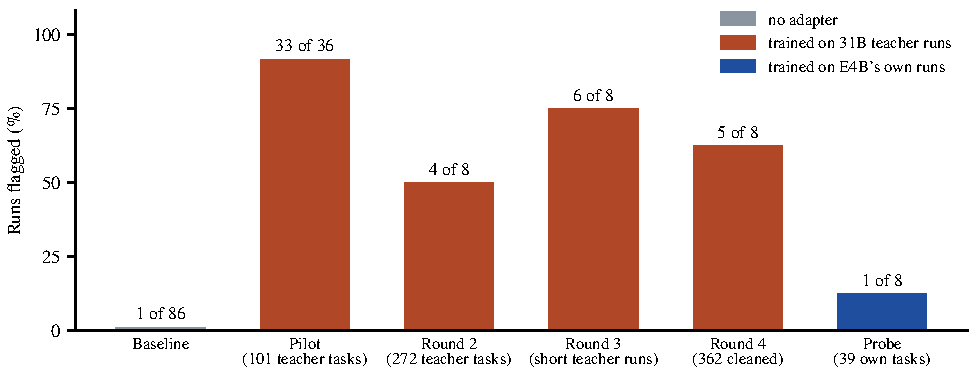
\includegraphics[width=\linewidth]{figs/screen.pdf}
\caption{Runs flagged by the loop screen. Adapters trained on the 31B teacher's runs are flagged on half or more of their runs; the probe trained on E4B's own runs on 1 of~8.}\label{fig:screen}
\end{figure}

More teacher data did not help: round 2 (272~tasks) aborted on 4 of the 8 screening tasks and round 3 (teacher runs of at most 25 budgeted tool calls) on 6. One cause was in the data. The harness nudges a model that ends a turn without a tool call, so successful teacher runs rarely stop at their fix: 28\% of all supervised calls came after the first \texttt{submit\_patch}, and the student learned to keep calling with nothing~changing.

The cleaned data cuts every verified run at its first \texttt{submit\_patch} that reports a non-empty patch, excludes runs that edit after that point or never submit successfully (88 of~450), and removes supervision from calls that repeat an earlier call with no edit in between. Round 4 (362 cleaned teacher tasks) still aborted on 5 of the 8 screening tasks: repeats fell from 69 to at most 31, but the student still searched for 37 to 57~calls and edited late or never. The 31B's search style, a median of~25 tool calls per success with long reading phases, is more than E4B can carry. Small models show the same gap when distilled from strong reasoners~\citep{learnability}.

\paragraph{The student's own runs.} A probe trained only on E4B's own verified successes (39~tasks from the training pools, about 9~calls each, cleaned the same way) passed the screen: 1 abort in 8, 6 to 17~calls per task, a first edit by call 4 to~10, and~3 of~8 resolved against the baseline's~2.

\paragraph{Held-out test.} Before opening any result on the 128~tasks outside the screen (82 out-of-distribution, 46 public), I fixed the next round and its evaluation. The larger round, the self-trained adapter, uses every base-model success verified by a fixed time (247~tasks from 221 repositories, 63 updates) and exactly the probe's recipe. The probe and the self-trained adapter are each compared with the baseline replicate under the rule above; with two candidates on one test set each needs a one-sided $p$ of~0.025 or less (Bonferroni). Neither passed (Table~\ref{tab:holdout}). Both moved the same way, by amounts the baseline replicate moves on its~own.


\paragraph{Learning from failures.} Most base-model runs fail and supervise nothing. Following privileged self-distillation for small agents \citep{sweladder,oprd}, a frozen copy of E4B rereads 460 model calls from 32 failed runs with a hint from the task's reference fix in its context: the files and functions the fix touches, plus the fix's hunks for files the run had already opened. Each generated token gets the advantage $A = \mathrm{clip}(\log q - \log p,\,-1,\,1)$, where $q$ is its probability under the hinted model and $p$ under the unhinted one, and the loss adds 0.1~times the sum of $A$ times the token's cross-entropy to the self-trained recipe, within the same 63 updates. Hints exist only in~training.

\begin{table}[t]
\centering
\caption{Held-out tasks. Wins, losses and the one-sided exact $p$ are against the baseline replicate on the 82 out-of-distribution tasks; loops are flagged runs, out-of-distribution then public.}\label{tab:holdout}
\small
\begin{tabular}{lrrrrrr}
\toprule
Adapter & Resolved of 82 & Wins & Losses & $p$ & Resolved of 46 & Loops \\
\midrule
Baseline replicate & 7 &  &  &  & 3 & 1, 0 \\
Probe (39 own tasks) & 9 & 3 & 1 & 0.31 & 6 & 3, 3 \\
Self-trained (247 own tasks) & 11 & 6 & 2 & 0.14 & 4 & 3, 1 \\
Self-trained with hints & 11 & 5 & 1 & 0.11 & 2 & 4, 3 \\
\bottomrule
\end{tabular}
\end{table}

On 64 fresh tasks with sound controls the base resolved 7, the self-trained adapter 9 and the hinted adapter 11. On the held-out tasks that lead of two did not carry over (Table~\ref{tab:holdout}), and I stopped after one~round.


\section{Release}\label{sec:release}

The release holds, without models and task contents: the environment fixes and the build script; the local scorer with its controls, the SWE-rebench adapter, the loop screen and the time projection; \texttt{cx} with its editor and regression tests; the capture proxy, the packing builder and the LoRA trainer; and the task lists (86 out-of-distribution, 3,046 training, 50 sound public) with each task's licence. The code is public at \mbox{\url{https://github.com/NikhilGogu/measure-first}} under the Apache License~2.0.


\section{Limitations}\label{sec:limits}

The public sound set covers two repositories. The out-of-distribution set is newer than the training pools but shares the SWE-rebench construction. Each comparison is one run per configuration at temperature 0.2. Thinking tokens are part of the training targets. \texttt{cx show} prints line numbers, which E4B copied into 137 of its 1,228~edits.


\phantomsection
\addcontentsline{toc}{section}{References}
\bibliographystyle{unsrtnat}
\bibliography{refs}
\end{document}
